\mysection{Division du travail}
Afin de simplifier le travail, celui-ci était divisé en plusieurs \textit{Work Packages}, chacun composé par des petites tâches. La division et ses respectives tâches peuvent être vues dans les sections \ref{Première Partie  - Lecture} à \ref{Cinquième Partie - Rédaction} suivantes.

\mysubsection{Première Partie  - Lecture}
La première partie consistait à lire l'article de WAN Yidong \cite{yidong}, qui explique d'une façon un peu simplifiée le problème et montre des façons de calculer les gains entre la tension des bus et la puissance réactive des charges, en utilisant des \textit{scripts} écrits en \gls{DPL} dans le logiciel PowerFactory et la création d'une matrice de gain.

Après la lecture de l'article, afin de comprendre le problème un peu mieux, la lecture de quelques parties de la thèse de Marjorie Cosson \cite{cosson:tel-01374469}  a été faite.
D'autres lectures supplémentaires ont été faites, \cite{farina2015model} et \cite{mariani2013controllo}. Ces articles utilisent le même réseaux que \cite{cosson:tel-01374469} et quelques données ont aidé pour la reconstruction du réseaux dans le PowerFactory.


\mysubsection{Deuxième Partie - Mise en Main}
Après la lecture des documents a commencé l'étude et la prise en main du logiciel DIgSILENT PowerFactory, en lisant et regardant les tutoriels sur l'internet, en faisant quelques petits exemples du logiciel afin d'apprendre a utiliser les outils nécessaires pour faire les tests proposés et après, faire la montage de la modèle du réseau dans le PowerFactory, dont le diagramme est montré dans la figure \ref{fig:Diagramme_du_reseaux}. 

\mysubsection{Troisième Partie - Programmation}
Pendant cette partie diverses scripts ont été crées en utilisant les langages MATLAB et Python:
\begin{itemize}
	\item Pour charger les valeurs de puissance des charges.
	\item Pour charger les valeurs de puissance des générateurs.
	\item Pour calculer les gains entre les bus et les générateurs.
	\item Pour faire des matrices de gains.
	\item Pour créer des événements de charges et générateurs, faire des simulations et prendre les résultats en graphiques.
\end{itemize}

\mysubsection{Quatrième Partie - Intégration}
	Pendant la quatrième partie, l'interface entre le PowerFactory et MATLAB a été requise a fin de créer une modèle de régulateur au simulink et utiliser dans le PowerFactory.
\pagebreak

\mysubsection{Cinquième Partie - Rédaction}
La cinquième partie consistait en élaborer des rapports et autres documents de description du projet, comme ce document par exemple.

\begin{figure}[H]
	\begin{center}	
		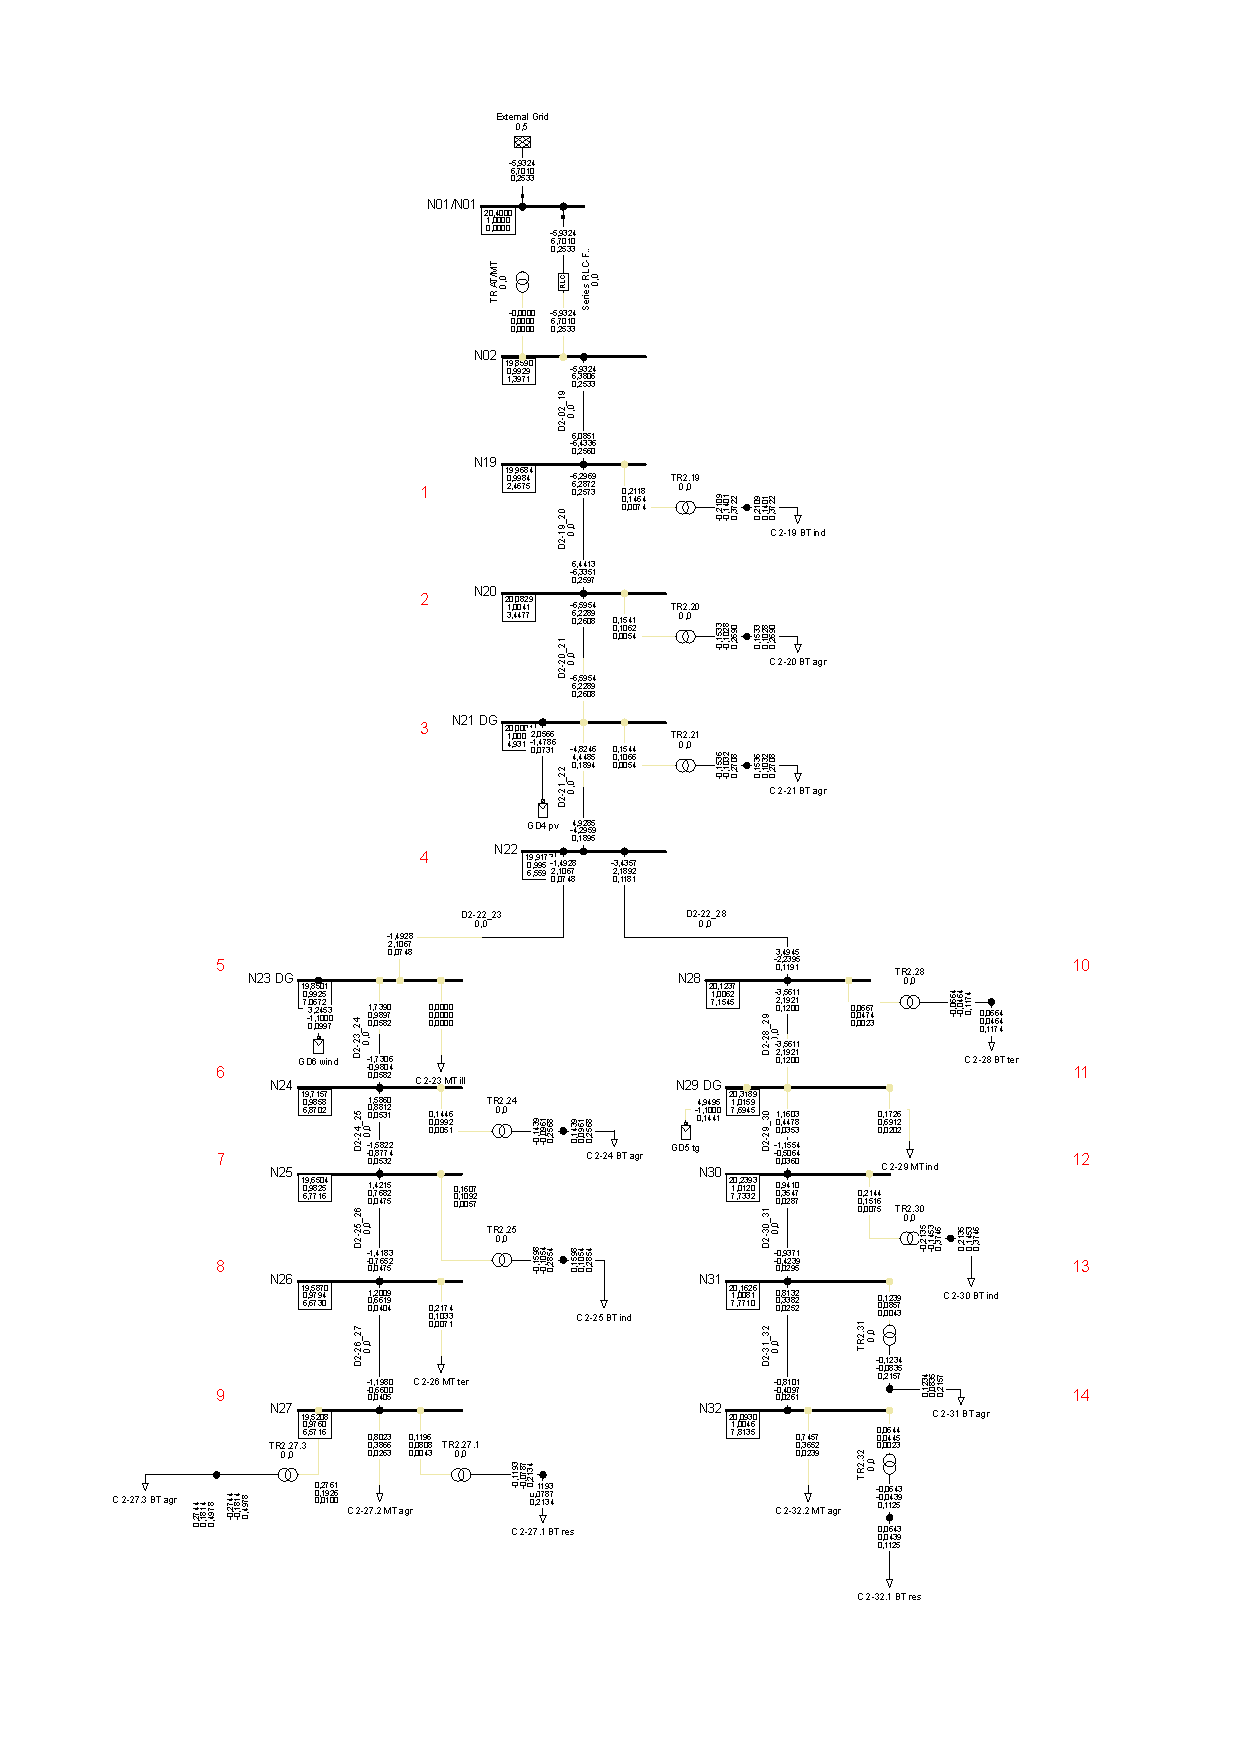
\includegraphics[width=\textwidth]{Division_du_travail/Diagramme_du_reseaux.pdf}
		\caption{Diagramme du reseaux}
		\label{fig:Diagramme_du_reseaux}
	\end{center}
\end{figure}
\newpage